% Options for packages loaded elsewhere
\PassOptionsToPackage{unicode}{hyperref}
\PassOptionsToPackage{hyphens}{url}
%
\documentclass[
  12pt,
]{article}
\title{County Level Predictors for Covid-19 Prevelance During the Introduction of Omnicron}
\author{Nathaniel Haulk\textsuperscript{1}}
\date{2021-12-07 14:29:41}

\usepackage{amsmath,amssymb}
\usepackage{lmodern}
\usepackage{setspace}
\usepackage{iftex}
\ifPDFTeX
  \usepackage[T1]{fontenc}
  \usepackage[utf8]{inputenc}
  \usepackage{textcomp} % provide euro and other symbols
\else % if luatex or xetex
  \usepackage{unicode-math}
  \defaultfontfeatures{Scale=MatchLowercase}
  \defaultfontfeatures[\rmfamily]{Ligatures=TeX,Scale=1}
\fi
% Use upquote if available, for straight quotes in verbatim environments
\IfFileExists{upquote.sty}{\usepackage{upquote}}{}
\IfFileExists{microtype.sty}{% use microtype if available
  \usepackage[]{microtype}
  \UseMicrotypeSet[protrusion]{basicmath} % disable protrusion for tt fonts
}{}
\makeatletter
\@ifundefined{KOMAClassName}{% if non-KOMA class
  \IfFileExists{parskip.sty}{%
    \usepackage{parskip}
  }{% else
    \setlength{\parindent}{0pt}
    \setlength{\parskip}{6pt plus 2pt minus 1pt}}
}{% if KOMA class
  \KOMAoptions{parskip=half}}
\makeatother
\usepackage{xcolor}
\IfFileExists{xurl.sty}{\usepackage{xurl}}{} % add URL line breaks if available
\IfFileExists{bookmark.sty}{\usepackage{bookmark}}{\usepackage{hyperref}}
\hypersetup{
  pdftitle={County Level Predictors for Covid-19 Prevelance During the Introduction of Omnicron},
  pdfauthor={Nathaniel Haulk1},
  hidelinks,
  pdfcreator={LaTeX via pandoc}}
\urlstyle{same} % disable monospaced font for URLs
\usepackage[margin=1in]{geometry}
\usepackage{longtable,booktabs,array}
\usepackage{calc} % for calculating minipage widths
% Correct order of tables after \paragraph or \subparagraph
\usepackage{etoolbox}
\makeatletter
\patchcmd\longtable{\par}{\if@noskipsec\mbox{}\fi\par}{}{}
\makeatother
% Allow footnotes in longtable head/foot
\IfFileExists{footnotehyper.sty}{\usepackage{footnotehyper}}{\usepackage{footnote}}
\makesavenoteenv{longtable}
\usepackage{graphicx}
\makeatletter
\def\maxwidth{\ifdim\Gin@nat@width>\linewidth\linewidth\else\Gin@nat@width\fi}
\def\maxheight{\ifdim\Gin@nat@height>\textheight\textheight\else\Gin@nat@height\fi}
\makeatother
% Scale images if necessary, so that they will not overflow the page
% margins by default, and it is still possible to overwrite the defaults
% using explicit options in \includegraphics[width, height, ...]{}
\setkeys{Gin}{width=\maxwidth,height=\maxheight,keepaspectratio}
% Set default figure placement to htbp
\makeatletter
\def\fps@figure{htbp}
\makeatother
% Make links footnotes instead of hotlinks:
\DeclareRobustCommand{\href}[2]{#2\footnote{\url{#1}}}
\setlength{\emergencystretch}{3em} % prevent overfull lines
\providecommand{\tightlist}{%
  \setlength{\itemsep}{0pt}\setlength{\parskip}{0pt}}
\setcounter{secnumdepth}{-\maxdimen} % remove section numbering
\newlength{\cslhangindent}
\setlength{\cslhangindent}{1.5em}
\newlength{\csllabelwidth}
\setlength{\csllabelwidth}{3em}
\newlength{\cslentryspacingunit} % times entry-spacing
\setlength{\cslentryspacingunit}{\parskip}
\newenvironment{CSLReferences}[2] % #1 hanging-ident, #2 entry spacing
 {% don't indent paragraphs
  \setlength{\parindent}{0pt}
  % turn on hanging indent if param 1 is 1
  \ifodd #1
  \let\oldpar\par
  \def\par{\hangindent=\cslhangindent\oldpar}
  \fi
  % set entry spacing
  \setlength{\parskip}{#2\cslentryspacingunit}
 }%
 {}
\usepackage{calc}
\newcommand{\CSLBlock}[1]{#1\hfill\break}
\newcommand{\CSLLeftMargin}[1]{\parbox[t]{\csllabelwidth}{#1}}
\newcommand{\CSLRightInline}[1]{\parbox[t]{\linewidth - \csllabelwidth}{#1}\break}
\newcommand{\CSLIndent}[1]{\hspace{\cslhangindent}#1}
\usepackage{geometry}
\geometry{verbose,letterpaper,margin=2.45cm}

% \usepackage[breaklinks=true,pdfstartview=FitH,citecolor=blue]{hyperref}
\hypersetup{colorlinks,%
	citecolor=blue,%
	filecolor=red,%
	linkcolor=blue,%
	urlcolor=red,%
	pdfstartview=FitH}

% \usepackage[T1]{fontenc}
% \usepackage[utf8]{inputenc}
% \usepackage{textgreek}
\usepackage{babel}
% % \usepackage{microtype}
% % \usepackage{amsmath}
\usepackage[osf]{libertine}
\usepackage{libertinust1math}
\usepackage{inconsolata}

\usepackage{longtable}

\usepackage{booktabs}

\usepackage{setspace}
% \doublespacing

% \setstretch{1.8999999999999999}

\usepackage{lineno}
% \linenumbers

\usepackage{flafter}
\usepackage{float}

% \renewcommand{\rmdefault}{cmr}

\usepackage[document]{ragged2e}

% % flush left while keep identation
% \makeatletter
% \newcommand\iraggedright{%
%   \let\\\@centercr\@rightskip\@flushglue \rightskip\@rightskip
%   \leftskip\z@skip}
% \makeatother
% \raggedright

% make pdf as default figure format
\DeclareGraphicsExtensions{.pdf,.png, %
    .jpg,.mps,.jpeg,.jbig2,.jb2,.JPG,.JPEG,.JBIG2,.JB2}
    
% \DeclareUnicodeCharacter{3B1}{\ensuremath{\alpha}}
% \DeclareUnicodeCharacter{3B2}{\ensuremath{\beta}}
% \DeclareUnicodeCharacter{0394}{$\Delta$}

\usepackage[labelsep=period]{caption}
\captionsetup{labelfont=bf}
% \usepackage{caption}
% \DeclareCaptionLabelSeparator{vline}{ \textbf{|} }
% \captionsetup{labelsep=vline, labelfont = {bf}}
\usepackage{booktabs}
\usepackage{longtable}
\usepackage{array}
\usepackage{multirow}
\usepackage{wrapfig}
\usepackage{float}
\usepackage{colortbl}
\usepackage{pdflscape}
\usepackage{tabu}
\usepackage{threeparttable}
\usepackage{threeparttablex}
\usepackage[normalem]{ulem}
\usepackage{makecell}
\usepackage{xcolor}
\ifLuaTeX
  \usepackage{selnolig}  % disable illegal ligatures
\fi

\begin{document}
\maketitle

% align only at left, not at right.
\renewcommand{\figurename}{{\textbf{Figure}}}
\renewcommand{\tablename}{{\textbf{Table}}}
% \iraggedright

\setstretch{1.5}
\footnotesize

\textsuperscript{1}Department of Biological Sciences, Louisiana State University, Baton Rouge, LA, USA

* \textbf{Corresponding author}, email: \href{mailto:nhaulk1@lsu.edu}{\nolinkurl{nhaulk1@lsu.edu}}; 232 Life Science Building, Baton Rouge, LA 70803

\normalsize

\textbf{Running headline}: Environment and species richness

\textbf{Abstract}: Your awesome abstract here.

\clearpage

\hypertarget{introduction}{%
\section{Introduction}\label{introduction}}

The first case of Covid-19 was recorded in the United States in January 22, 2020 according to the CDC. As of December 5, 2021, the United States has reported more than 780000 deaths due to Covid-19, more than any other country (\protect\hyperlink{ref-new_york_times_coronavirus_2021}{New York Times 2021}). Initially, non-pharmaceutical methods were used to help stop the spread of Covid-19, including the closing of many public spaces, encouraging social distancing, and encouraging the use of masks to help reduce transmission rates. Through time, social distancing and mask mandate policies changed as Covid-19 became the new norm, leading to patterns of increasing and decreasing Covid-19 rates in the United States (\protect\hyperlink{ref-rebeiro_impact_2021}{Rebeiro et al. 2021}). The current widespread availability of vaccines helping to fight Covid-19 has also helped to reduce the overall transmission and resulting mortality (\protect\hyperlink{ref-haas_infections_2021}{Haas et al. 2021}). Transmission and Covid-19 rates have increased post vaccination due to mutations in spike proteins that have allowed for new variants of COVID-19 to spread \protect\hyperlink{ref-monajjemi_delta_nodate}{Monajjemi et al.} (\protect\hyperlink{ref-monajjemi_delta_nodate}{n.d.}). As of December 5th, 2021, the Delta variant, is the most common strain of COVID-19, representing more than 99 percent of cases (\protect\hyperlink{ref-cdc_covid_2020}{CDC 2020}).

Mask mandates, social distancing, and vaccination have all been proven to reduce the transmission of Covid-19 (\protect\hyperlink{ref-ferguson_report_2020}{Ferguson et al. 2020}, \protect\hyperlink{ref-lyu_community_2020}{Lyu and Wehby 2020}, \protect\hyperlink{ref-nguyen_mask_2021}{Nguyen 2021}, \protect\hyperlink{ref-haas_infections_2021}{Haas et al. 2021}). Areas that adopted the use of masks early tended to have lower overall COVID-19 rates compared to those that did not. Given the efficacy of masks preventing transmission as well as the high-availability to everyone, masks have been one of the best tools in fighting the spread of Covid-19 (\protect\hyperlink{ref-rebeiro_impact_2021}{Rebeiro et al. 2021}). Despite the clear benefits, masks have been met with much opposition across the United States, especially in politically conservative leaning counties (\protect\hyperlink{ref-kahane_politicizing_2021}{Kahane 2021}, \protect\hyperlink{ref-he_why_2021}{He et al. 2021}). These counties tend to be more rural and more against mask mandates than their urban counterparts (\protect\hyperlink{ref-pro_us_2021}{Pro et al. 2021}).

Spatial Heterogeneity, or the uneven distribution of populations across space, is important for predicting disease dynamics in pathogens like Covid-19. Areas with low spatial heterogeneity tend to be better environments for a disease to persist when compared to high spatial heterogeneous environments (\protect\hyperlink{ref-hagenaars_spatial_2004}{Hagenaars et al. 2004}). Populations with higher densities tend to have higher disease spread assuming the disease transmission is not based on frequency of contact (\protect\hyperlink{ref-scott_impact_1988}{Scott 1988}). Density dependent disease like Covid-19 should therefore have a harder time spreading in rural areas with higher heterogeneity and lower population densities. However, with resistance to preventative measures such as masks and vaccines, cases may be higher in rural areas than their urban counterparts (\protect\hyperlink{ref-sun_rural-urban_2021}{Sun and Monnat 2021}).

With changes in population density and spacial spread, the basic reproductive number, \(R_0\), should change as a result. The basic reproductive number represents the number of predicted infections that can result from one infection (\protect\hyperlink{ref-delamater_complexity_2019}{Delamater et al. 2019}). While studies have already looked into how \(R_0\) changes by county, no recent studies have looked at the effective reproductive number on a county level (\protect\hyperlink{ref-ives_estimating_2021}{Ives and Bozzuto 2021}). More importantly, not much is yet known about the new Omicron variant first introduced into the US on December 1, 2021. The Omicron variant is predicted to be more infectious than previous variants of Covid-19 and is predicted to be more resistant to the vaccines we currently have available (\protect\hyperlink{ref-cdc_omicron_2021}{CDC 2021a}). The Reproductive number of the Omicron variant is not calculable at such a low prevalence due to the lack of data. However, predictions on how the new variant will spread provides vital information on preventing new infections and reducing overall mortality.

While data is presented on county-level Covid-19 rates, few studies have taken this further to investigate the how the infection rates in urban and rural areas compare. With the Omicron variant just recently emerging, no studies have yet to be published examining the predicted rate of spread. In this study, I seek to investigate the total infection prevalence per county. I also compare the prevalence per county in rural and urban areas, as well as those with and without mask mandates. Finally, I seek to use previous predictions of R0 to calculate Rt in its current state. Using these current Rt values, I then infer predicted Rt values for Omicron for each county to highlight at-risk counties.

\hypertarget{methods}{%
\section{Methods}\label{methods}}

All code and graphs were written using the programming language R and maps of the United States were modeled using the package USmaps(\protect\hyperlink{ref-lorenzo_usmap_2021}{Lorenzo 2021}, \protect\hyperlink{ref-r_core_team_r_2021}{R Core Team 2021}). For data on Covid-19 cases by county, I used the time series data provided by the New York Times (\protect\hyperlink{ref-new_york_times_coronavirus_2021}{New York Times 2021}). For total population estimates, I used US Census data predictions for 2021 (\protect\hyperlink{ref-united_states_census_bureau_county_2021}{United States Census Bureau 2021a}). Total cases were mapped out as the number of cases in each county divided by the total population to get the total percentage of infections (Figure \ref{fig:fig1}). Rolling averages were mapped out based on reported cases within the last 30 days (Figure \ref{fig:fig2}). Mask mandate data used was collected in July of 2020(\protect\hyperlink{ref-wright_tracking_2020}{Wright et al. 2020}). Data from the early infection was chosen and graphed to show how early responses to Covid-19 have led difference in the total percentage of cases (Figure \ref{fig:fig3}). A t-test was performed to test the significance between the two groups and bar graph was made for visualization (Figure \ref{fig:fig4}). Rural data was graphed using two criteria, based on HRSA classifications and the census Bureaus classifications of urban and rural areas (\protect\hyperlink{ref-hrsa_defining_2021}{HRSA 2021}, \protect\hyperlink{ref-united_states_census_bureau_2010_2021}{United States Census Bureau 2021b}). Both were graphed as a map of the US to show county classification as well as a bar graph to compare the average total case percentage (Figure \ref{fig:fig5}; Figure \ref{fig:fig6}). An ANOVA test was performed on the data classified based on the Census Bureau Data distinction of urban and rural to test for significance. A t-test was performed on the data classified based on the HRSA distinction of urban and rural to test for significance. R Vaccine data was collected from the CDC to calculate the proportion of susceptible individuals (\protect\hyperlink{ref-cdc_covid-19_2021}{CDC 2021b}).

The effective reproductive number (\(R_t\)) was calculated using basic reproductive values(\(R_0\)) for each county predicted in a previous studies (Figure \ref{fig:fig7}) (\protect\hyperlink{ref-ives_estimating_2021}{Ives and Bozzuto 2021}) . Using previous models and calculations of \(R_0\), the formula
\[R_0 = \frac{\beta*\lambda}{(\gamma+\mu+\epsilon+\sigma)*(\tau+\mu)}\]
was used to calculate the \(\beta\) value, or the transmission rate, per county (see Table \ref{tab:suptable1} for parameter descriptions) (\protect\hyperlink{ref-ahmed_mathematical_2021}{Ahmed et al. 2021}). Beta values were than used to calculate using the formula
\[R_t = (1-p)*\frac{S}{N}*\frac{\beta*\lambda}{(\gamma+\mu+\epsilon+\sigma)*(\tau+\mu)}\]
where S represents individuals Suscpetible to the disease and N represents the total population size in that count. Parameter p represents the proportion of vaccinated individuals per county (\protect\hyperlink{ref-cdc_covid-19_2021}{CDC 2021b}). The effective reproductive number for the Omicron was then calculated using the same formula, with higher overall transmission rates and lower mask mandate usage to reflect the increase in R0 seen when the Delta variant of Covid-19 was first introduced into the United States (\protect\hyperlink{ref-liu_reproductive_2021}{Liu and Rocklöv 2021}).

\hypertarget{results}{%
\section{Results}\label{results}}

\hypertarget{figures}{%
\paragraph{Figures}\label{figures}}

Insert figure by code chunk. And cross-ref it back as Figure \ref{fig:fig1}.



\begin{figure}[H]

{\centering 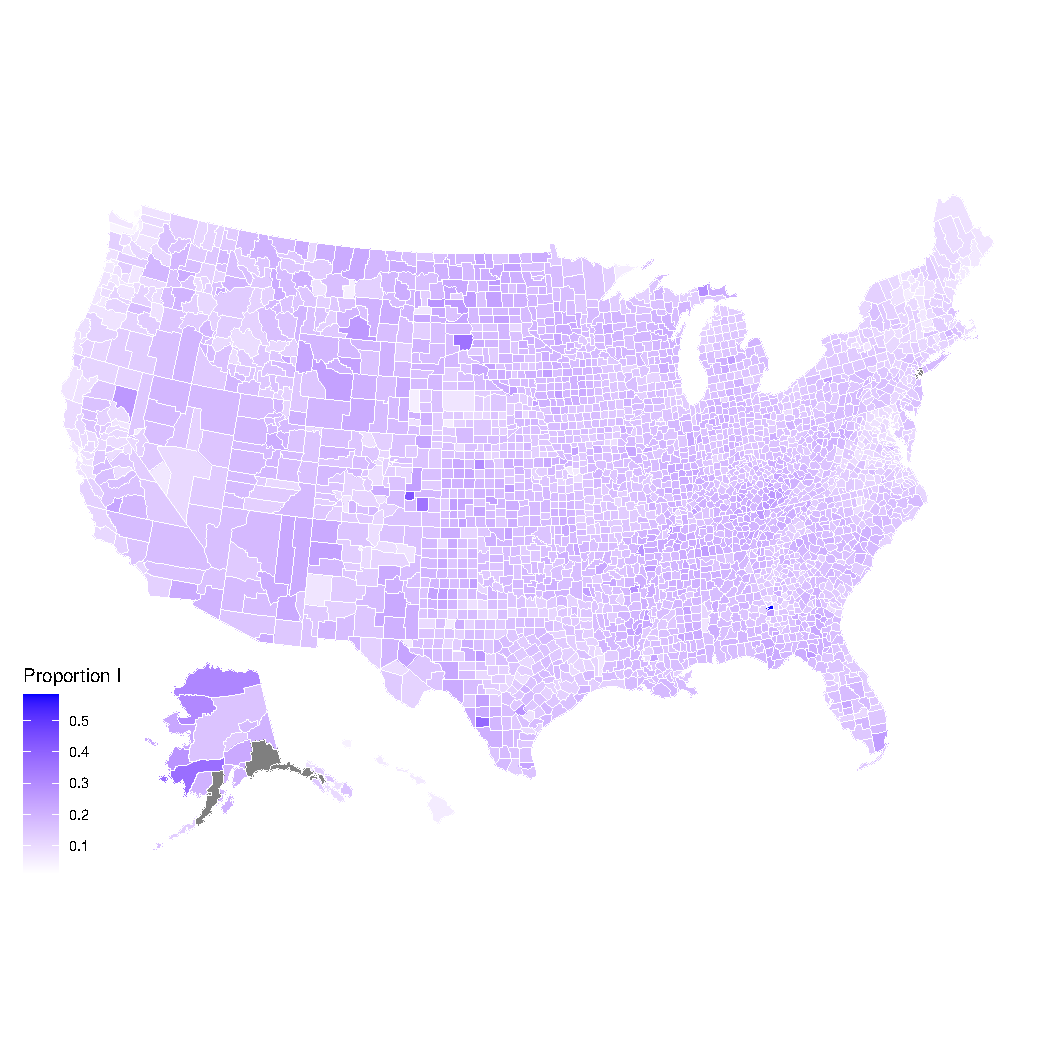
\includegraphics{Final-Manuscript_files/figure-latex/fig1-1} 

}

\caption{\textbf{No - or \_ in the caption ref.} No space at the end of this line!}\label{fig:fig1}
\end{figure}



\begin{figure}[H]

{\centering 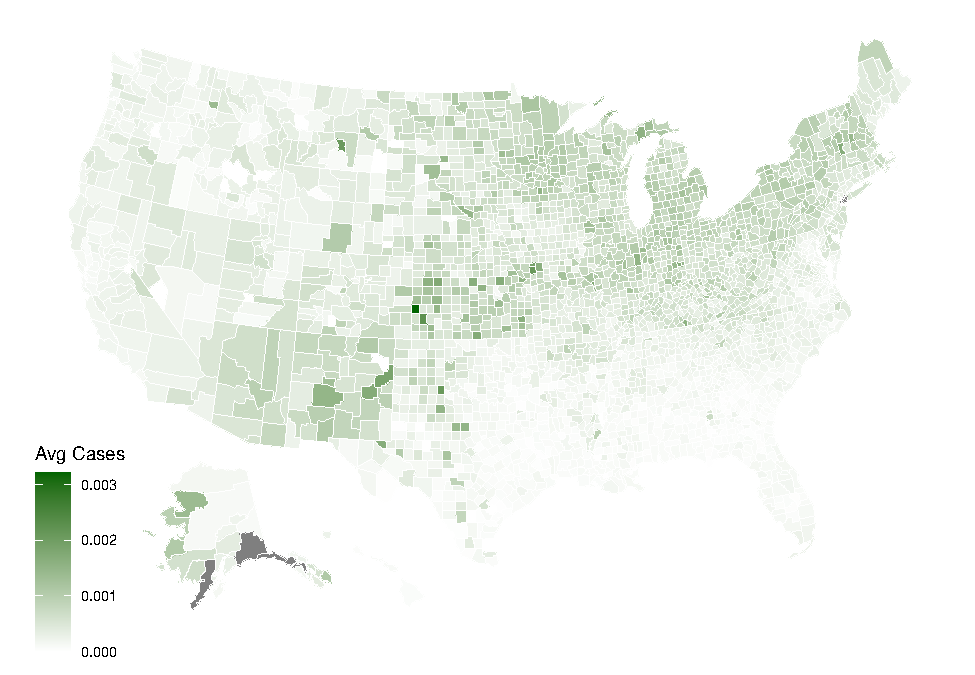
\includegraphics[width=0.7\linewidth,]{Final-Manuscript_files/figure-latex/fig2, -1} 

}

\caption{\textbf{No - or \_ in the caption ref.} No space at the end of this line!}(\#fig:fig2, )
\end{figure}







\begin{figure}[H]

{\centering 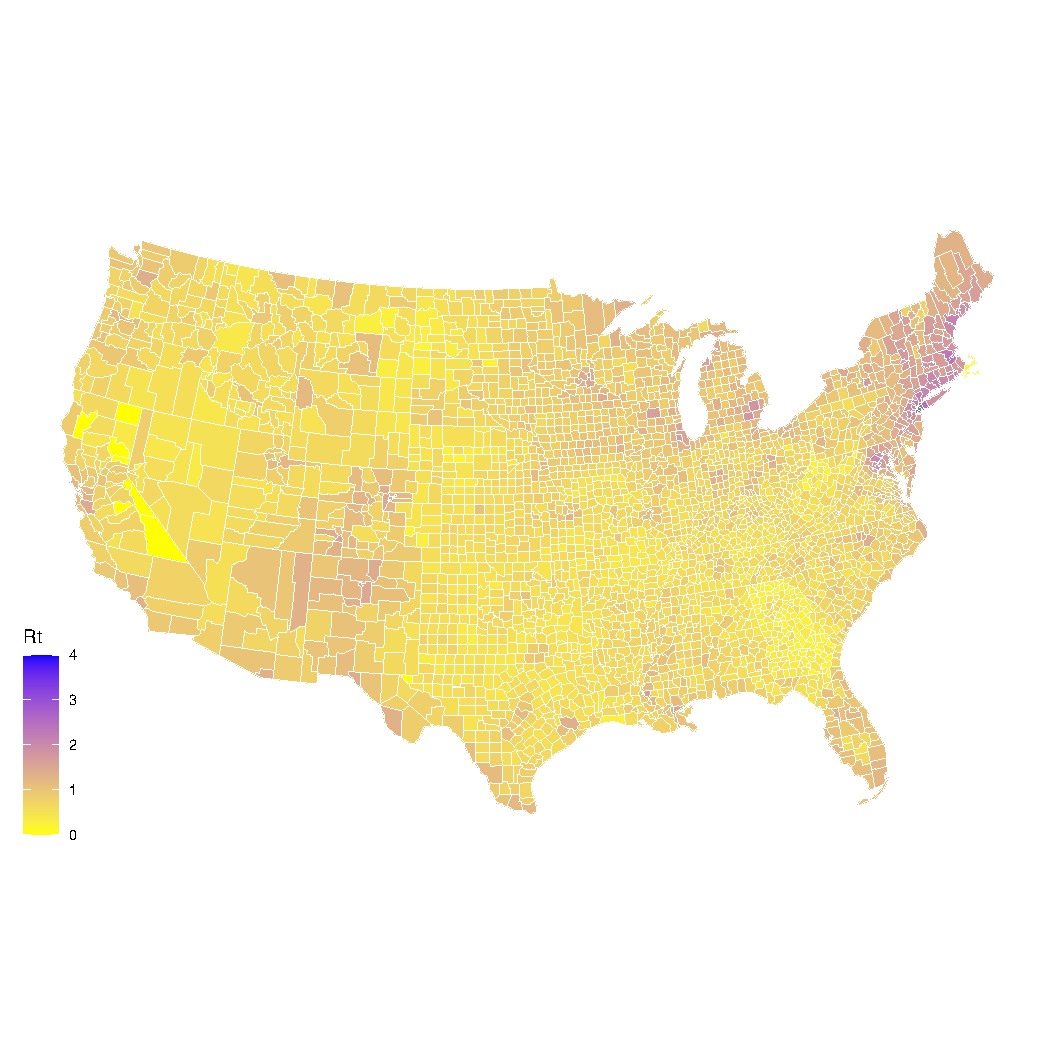
\includegraphics{Final-Manuscript_files/figure-latex/fig7-1} 

}

\caption{\textbf{No - or \_ in the caption ref.} No space at the end of this line!}\label{fig:fig7}
\end{figure}



\begin{figure}[H]

{\centering 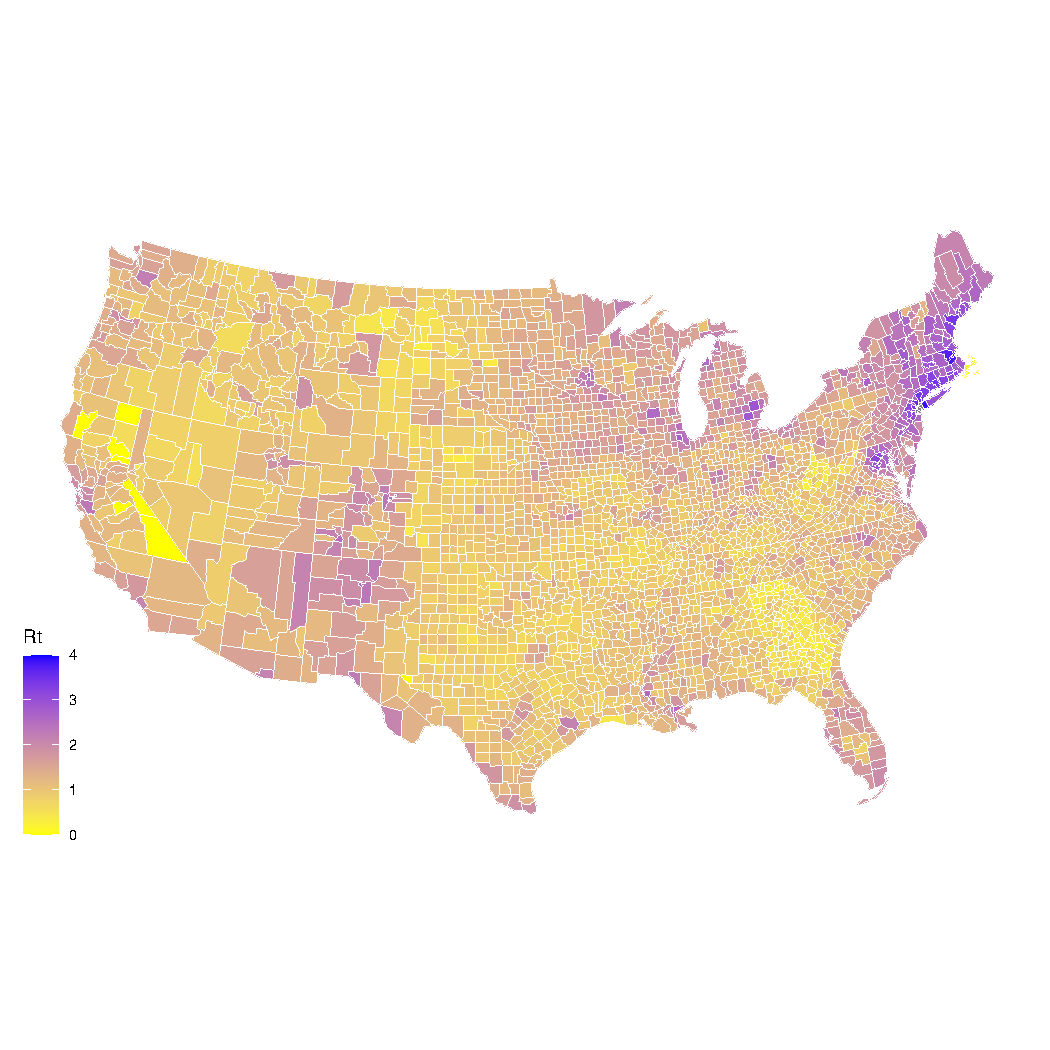
\includegraphics{Final-Manuscript_files/figure-latex/fig8-1} 

}

\caption{\textbf{No - or \_ in the caption ref.} No space at the end of this line!}\label{fig:fig8}
\end{figure}

\hypertarget{discussion}{%
\section{Discussion}\label{discussion}}

I used current data on Covid-19, effective

Focus on these counties

Masks do work.

Vaccine data all over the place.

Potential error

\hypertarget{conclusion}{%
\section{Conclusion}\label{conclusion}}

\hypertarget{references}{%
\section{References}\label{references}}

\hypertarget{refs}{}
\begin{CSLReferences}{1}{0}
\leavevmode\vadjust pre{\hypertarget{ref-ahmed_mathematical_2021}{}}%
Ahmed, I., G. U. Modu, A. Yusuf, P. Kumam, and I. Yusuf. 2021. A mathematical model of {Coronavirus} {Disease} ({COVID}-19) containing asymptomatic and symptomatic classes. Results in Physics 21:103776.

\leavevmode\vadjust pre{\hypertarget{ref-cdc_covid_2020}{}}%
CDC. 2020, March. {COVID} {Data} {Tracker}.

\leavevmode\vadjust pre{\hypertarget{ref-cdc_omicron_2021}{}}%
CDC. 2021a, December. Omicron {Variant}: {What} {You} {Need} to {Know}.

\leavevmode\vadjust pre{\hypertarget{ref-cdc_covid-19_2021}{}}%
CDC. 2021b, December. {COVID}-19 {Vaccinations} in the {United} {States},{County} {\textbar} {Data} {\textbar} {Centers} for {Disease} {Control} and {Prevention}.

\leavevmode\vadjust pre{\hypertarget{ref-delamater_complexity_2019}{}}%
Delamater, P. L., E. J. Street, T. F. Leslie, Y. T. Yang, and K. H. Jacobsen. 2019. Complexity of the {Basic} {Reproduction} {Number} ({R0}). Emerging Infectious Diseases 25:1--4.

\leavevmode\vadjust pre{\hypertarget{ref-ferguson_report_2020}{}}%
Ferguson, N., D. Laydon, G. Nedjati Gilani, N. Imai, K. Ainslie, M. Baguelin, S. Bhatia, A. Boonyasiri, Z. Cucunuba Perez, G. Cuomo-Dannenburg, A. Dighe, I. Dorigatti, H. Fu, K. Gaythorpe, W. Green, A. Hamlet, W. Hinsley, L. Okell, S. Van Elsland, H. Thompson, R. Verity, E. Volz, H. Wang, Y. Wang, P. Walker, P. Winskill, C. Whittaker, C. Donnelly, S. Riley, and A. Ghani. 2020. Report 9: {Impact} of non-pharmaceutical interventions ({NPIs}) to reduce {COVID19} mortality and healthcare demand. Imperial College London.

\leavevmode\vadjust pre{\hypertarget{ref-haas_infections_2021}{}}%
Haas, E. J., J. M. McLaughlin, F. Khan, F. J. Angulo, E. Anis, M. Lipsitch, S. R. Singer, G. Mircus, N. Brooks, M. Smaja, K. Pan, J. Southern, D. L. Swerdlow, L. Jodar, Y. Levy, and S. Alroy-Preis. 2021. Infections, hospitalisations, and deaths averted via a nationwide vaccination campaign using the {Pfizer}--{BioNTech} {BNT162b2} {mRNA} {COVID}-19 vaccine in {Israel}: A retrospective surveillance study. The Lancet Infectious Diseases.

\leavevmode\vadjust pre{\hypertarget{ref-hagenaars_spatial_2004}{}}%
Hagenaars, T. J., C. A. Donnelly, and N. M. Ferguson. 2004. Spatial heterogeneity and the persistence of infectious diseases. Journal of Theoretical Biology 229:349--359.

\leavevmode\vadjust pre{\hypertarget{ref-he_why_2021}{}}%
He, L., C. He, T. L. Reynolds, Q. Bai, Y. Huang, C. Li, K. Zheng, and Y. Chen. 2021. Why do people oppose mask wearing? {A} comprehensive analysis of {U}.{S}. Tweets during the {COVID}-19 pandemic. Journal of the American Medical Informatics Association : JAMIA 28:1564--1573.

\leavevmode\vadjust pre{\hypertarget{ref-hrsa_defining_2021}{}}%
HRSA. 2021, October. Defining {Rural} {Population}. Text.

\leavevmode\vadjust pre{\hypertarget{ref-ives_estimating_2021}{}}%
Ives, A. R., and C. Bozzuto. 2021. Estimating and explaining the spread of {COVID}-19 at the county level in the {USA}. Communications Biology 4:60.

\leavevmode\vadjust pre{\hypertarget{ref-kahane_politicizing_2021}{}}%
Kahane, L. H. 2021. Politicizing the {Mask}: {Political}, {Economic} and {Demographic} {Factors} {Affecting} {Mask} {Wearing} {Behavior} in the {USA}. Eastern Economic Journal 47:163--183.

\leavevmode\vadjust pre{\hypertarget{ref-liu_reproductive_2021}{}}%
Liu, Y., and J. Rocklöv. 2021. The reproductive number of the {Delta} variant of {SARS}-{CoV}-2 is far higher compared to the ancestral {SARS}-{CoV}-2 virus. Journal of Travel Medicine 28:taab124.

\leavevmode\vadjust pre{\hypertarget{ref-lorenzo_usmap_2021}{}}%
Lorenzo, P. D. 2021. Usmap: {US} {Maps} {Including} {Alaska} and {Hawaii}.

\leavevmode\vadjust pre{\hypertarget{ref-lyu_community_2020}{}}%
Lyu, W., and G. L. Wehby. 2020. Community {Use} {Of} {Face} {Masks} {And} {COVID}-19: {Evidence} {From} {A} {Natural} {Experiment} {Of} {State} {Mandates} {In} {The} {US}. Health Affairs 39:1419--1425.

\leavevmode\vadjust pre{\hypertarget{ref-monajjemi_delta_nodate}{}}%
Monajjemi, M., F. Kandemirli, and F. Mollaamin. (n.d.). Delta {Variant} of {Covid}-19 {Study}, and {Why} it is a {Concern}: {An} {Overview}:14.

\leavevmode\vadjust pre{\hypertarget{ref-new_york_times_coronavirus_2021}{}}%
New York Times. 2021, December. Coronavirus ({Covid}-19) {Data} in the {United} {States}. The New York Times.

\leavevmode\vadjust pre{\hypertarget{ref-nguyen_mask_2021}{}}%
Nguyen, M. 2021. Mask {Mandates} and {COVID}-19 {Related} {Symptoms} in the {US}. ClinicoEconomics and Outcomes Research: CEOR 13:757--766.

\leavevmode\vadjust pre{\hypertarget{ref-pro_us_2021}{}}%
Pro, G., K. Schumacher, R. Hubach, N. Zaller, Z. Giano, R. Camplain, C. Camplain, S. Haberstroh, J. A. Baldwin, and D. L. Wheeler. 2021. {US} trends in mask wearing during the {COVID}-19 pandemic depend on rurality. Rural Remote Health:6596--6596.

\leavevmode\vadjust pre{\hypertarget{ref-r_core_team_r_2021}{}}%
R Core Team. 2021. R: {A} {Language} and {Environment} for {Statistical} {Computing}. R Foundation for Statistical Computing, Vienna, Austria.

\leavevmode\vadjust pre{\hypertarget{ref-rebeiro_impact_2021}{}}%
Rebeiro, P. F., D. M. Aronoff, and M. K. Smith. 2021. The {Impact} of {State} {Mask}-{Wearing} {Requirements} on the {Growth} of {Coronavirus} {Disease} 2019 {Cases}, {Hospitalizations}, and {Deaths} in the {United} {States}. Clinical Infectious Diseases 73:1703--1706.

\leavevmode\vadjust pre{\hypertarget{ref-scott_impact_1988}{}}%
Scott, M. E. 1988. The {Impact} of {Infection} and {Disease} on {Animal} {Populations}: {Implications} for {Conservation} {Biology}. Conservation Biology 2:40--56.

\leavevmode\vadjust pre{\hypertarget{ref-sheikh_sars-cov-2_2021}{}}%
Sheikh, A., J. McMenamin, B. Taylor, and C. Robertson. 2021. {SARS}-{CoV}-2 {Delta} {VOC} in {Scotland}: Demographics, risk of hospital admission, and vaccine effectiveness. The Lancet 397:2461--2462.

\leavevmode\vadjust pre{\hypertarget{ref-sun_rural-urban_2021}{}}%
Sun, Y., and S. M. Monnat. 2021. Rural-urban and within-rural differences in {COVID}-19 vaccination rates. The Journal of Rural Health n/a.

\leavevmode\vadjust pre{\hypertarget{ref-united_states_census_bureau_county_2021}{}}%
United States Census Bureau. 2021a. County {Population} {Totals}: 2010-2020.

\leavevmode\vadjust pre{\hypertarget{ref-united_states_census_bureau_2010_2021}{}}%
United States Census Bureau. 2021b, October. 2010 {Census} {Urban} and {Rural} {Classification} and {Urban} {Area} {Criteria}.

\leavevmode\vadjust pre{\hypertarget{ref-wright_tracking_2020}{}}%
Wright, A. L., G. Chawla, L. Chen, and A. Farmer. 2020. Tracking {Mask} {Mandates} {During} the {Covid}-19 {Pandemic}. SSRN Electronic Journal.

\end{CSLReferences}

\clearpage

\setcounter{page}{0}
\pagenumbering{arabic}
\setcounter{page}{1}

\setcounter{figure}{0}
\setcounter{table}{0}
\renewcommand {\thetable}{S\arabic{table}}
\renewcommand {\thefigure}{S\arabic{figure}}

\hypertarget{supporting-information}{%
\section{Supporting Information}\label{supporting-information}}

\hypertarget{tables}{%
\subsection{Tables}\label{tables}}

\begin{longtable}[]{@{}lcc@{}}
\caption{\label{tab:suptable1} Parameter descriptions and values used to calculate \(R_0\) (\protect\hyperlink{ref-ahmed_mathematical_2021}{Ahmed et al. 2021}).}\tabularnewline
\toprule
Parameter & Value & Description \\
\midrule
\endfirsthead
\toprule
Parameter & Value & Description \\
\midrule
\endhead
\(\beta\) & Varies & Transmission rate \\
\(\lambda\) & \(.0025\) & Births into system \\
\(\gamma\) & \(2.01*10^{-4}\) & Transfer from the exposed class to the quarantined class \\
\(\mu\) & \(.0015\) & Natural Mortality Rate \\
\(\epsilon\) & \(.45\) & Transfer from the exposed class to the symptomatic infected class \\
\(\sigma\) & \(.067\) & Transfer from the exposed class to the asymptomatic infected class \\
\(\tau\) & \(2*10^{-4}\) & Transfer from the susceptible class to the quarantine class \\
p & Varies & Proportion vaccinated \\
\bottomrule
\end{longtable}

\end{document}
